\section{Graphen\label{sec:sgwt:graphs}}
\rhead{Graphen}

Unsere Grundlage, auf der wir die SGWT aufbauen wollen, stellen Graphen dar. 
Ein Graph $G$ setzt sich aus Kanten $E$ und Knoten $V$ zusammen.
\begin{equation*}
G = \{V, E\}
\end{equation*}
Eine Kante verbindet dabei jeweils zwei Knoten miteinander.
\begin{equation*}
E = (V_1, V_2)
\end{equation*}

\begin{figure}
    \centering
    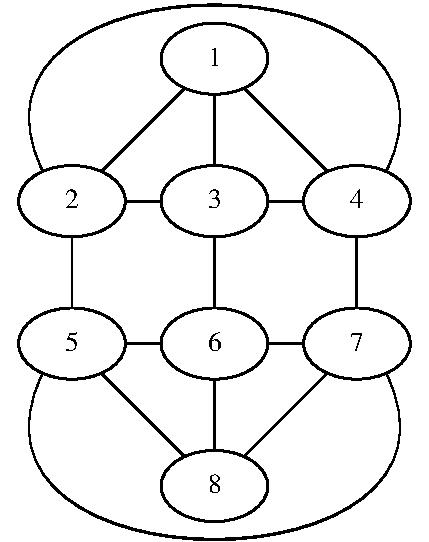
\includegraphics{papers/sgwt/images/sphere-graph.pdf}
    \caption{Graph-Darstellung einer Kugel. \label{sgwt:sphere:graph}}
\end{figure}
